\documentclass{beamer}
\usepackage[ngerman]{babel}
\usepackage[utf8]{inputenc}
\usepackage{graphicx}
\usepackage{amsmath}
\usepackage{amssymb}
\usepackage{dsfont}
\usepackage[T1]{fontenc}
\usepackage{pstricks}
\usepackage{pst-node}
%\usepackage[english]{babel}
%\usepackage[fixlanguage]{babelbib}
\usepackage{multimedia}


\usetheme{Warsaw}

\title[Einführung in DEC]{Einführung in das Kalkül diskreter Differentialformen}
\author{Ingo Nitschke}
\institute{IWR - TU Dresden}

\beamertemplatenavigationsymbolsempty

\newcommand{\R}{\mathds{R}}
\newcommand{\eps}{\varepsilon}
\newcommand{\qqquad}{\qquad\qquad}
\newcommand{\rot}{\text{rot}}
\newcommand{\sgn}{\text{sgn}}
\renewcommand{\div}{\text{div}}


\begin{document}

 \frame{ \titlepage }
 \frame {
    \frametitle{Content}
    \tableofcontents
  }

  \section{Primär- und Dualkomplexe}
  \frame {
    \begin{block}{Ein \( p \)-\textbf{Simplex} ist die konvexe Hülle von \( p+1 \) geometrisch unabhängigen Punkten (\textbf{Knoten}, \textbf{Vertices})}
      \[ \sigma^{p} := \left\{  x \in \R^{N} \middle| x = \sum_{i=0}^{p}\mu^{i}v_{i} \text{ wobei } \mu^{i} \ge 0  \text{ und } \sum_{i=0}^{p}\mu^{i} = 1 \right\}\]
    \end{block}
    \textbf{Geometrisch unabhängig} heißt, dass die \( p \) Vektoren \( v_{1} - v_{0}, \ldots,  v_{p} - v_{0} \) linear unabhängig sind.
    \begin{block}{Beispiel für \( \sigma^{2} \), \( \sigma^{1} \) und \( \sigma^{0} \) }
      \centering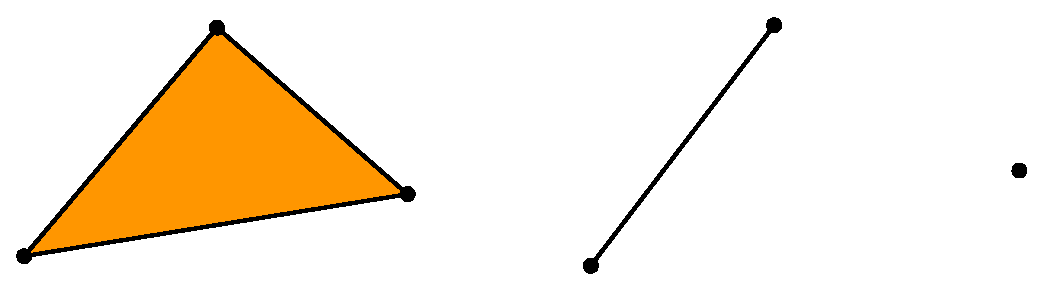
\includegraphics[width=0.9\textwidth]{bilder/inkscape/DreieckLiniePunkt.eps}
    \end{block}
  }

  \begin{frame}
    \begin{block}{Ein \textbf{Simplizialkomplex} \( K \) der \textbf{Dimension} \( n \) ist eine Menge von Simplizes \( \left\{\sigma^{p} \in \R^{N} \middle| 0 \le p \le n \le N \right\}\), so dass}
      \begin{enumerate}[(i)]
        \item \( \forall \sigma^{r} \prec \sigma^{p} :\quad \sigma^{r} \in K \qquad (0 \le r \le p) \)
        \item für alle \( \sigma^{r} := \sigma^{p} \cap \sigma^{q} \) gilt \( \qquad (0 \le r \le \min\{p,q\}) \)
              \begin{enumerate}[(a)]
                \item entweder \( \sigma^{r} \prec \sigma^{p}\) und  \( \sigma^{r} \prec \sigma^{q}\)
                \item oder \( \sigma^{r} = \emptyset \)
              \end{enumerate}
      \end{enumerate}
    \end{block}
    D.h. z.B. hängende Knoten sind nicht zulässig.
    \begin{block}{Das \textbf{Polytop} von \( K \) ist (der zu Grunde liegende Raum)}
      \[ |K| := \bigcup_{\sigma \in K} \sigma \]
    \end{block}
    (Andersherum heißt \( K \) eine \textbf{Triangulation} von \( |K| \))\\ 
    Achtung: \( |K| \) liegt nur für \textbf{flache} (\textbf{lineare}) \( K \) in einem affinen \( n \)-dim. Untervektoraum des \( \R^{N} \).
  \end{frame}

  \begin{frame}
    \begin{block}{Diskretisierung einer Mannigfaltigkeit \( M \)}
      \begin{itemize}
        \item Wir wollen nicht die Kartengebiete auf der Mannigfaltigkeit diskretisieren.
        \item Die \( n \)-Mannigfaltigkeit wird in den \( \R^{N} \) eingebettet.
        \item Wir setzen dann nur voraus, dass \( \sigma^{0}_{M} = \sigma^{0}_{K} \)
      \end{itemize}
    \end{block}
    \begin{block}{Beispiel}
      \centering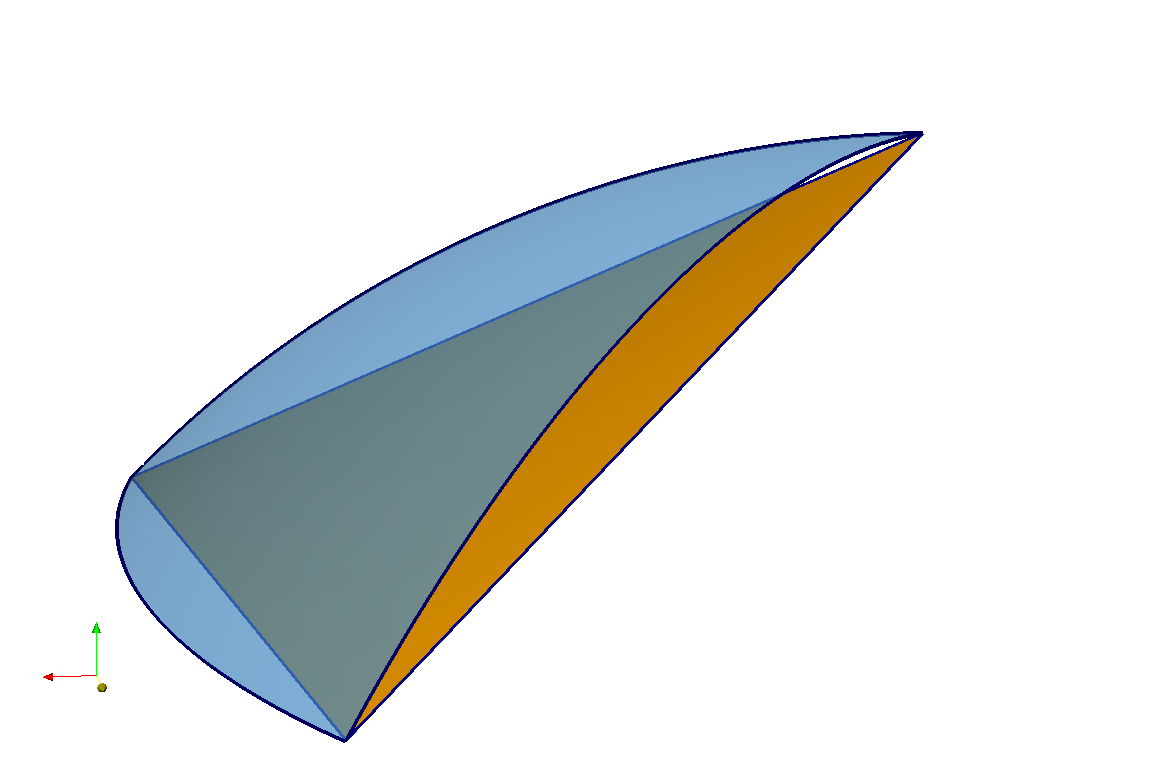
\includegraphics[width=0.5\textwidth]{bilder/paraview/abstractSimplex.png}
    \end{block}
  \end{frame}

  \begin{frame}
    \begin{block}{\textbf{Orientierter mannigfaltigartiger Simplizialkomplex} \( K \) (\textbf{Primärgitter})}
      \begin{description}
        \item[orientiert:] \( \sgn(\sigma^{n}_{1}, \sigma^{n}_{2}) = +1 \) für \( \sigma^{n}_{1} \cap \sigma^{n}_{2} \ne \emptyset \)
        \item[mannigfaltigartig:] \( |K| \) ist eine \( C^{0} \)-Mannigfaltigkeit
      \end{description}
    \end{block}
  \end{frame}
 

\end{document}
